\documentclass[]{article}
\usepackage{graphicx}
%opening
\title{}
\author{}

\begin{document}

%\maketitle

\section{Synthetic dataset 1}
\begin{table*}[h]
\caption{NMSE Results (M=5)} \label{table:basisfunction}
\vspace{-.0in}
\begin{center}
\begin{tabular}{|c|c|c|}
\hline
Methods & NMSE in [-1, 7]& NMSE in [0, 6] \\
\hline 
\hline
EigenGP (ARD) &  $ 0.019 \pm 0.0018$ & $0.012\pm0.0031$\\
\hline
EigenGP (ARD+linear)& $0.041\pm0.0051$  & $0.0080\pm0.0012$\\
\hline 
\end{tabular}
\end{center}
\vspace{-.0in}
\end{table*}
The ARD+linear model does not perform well outside the range of training data but performs 
well inside. The following figure (one run of the composite model) illustrates this result.

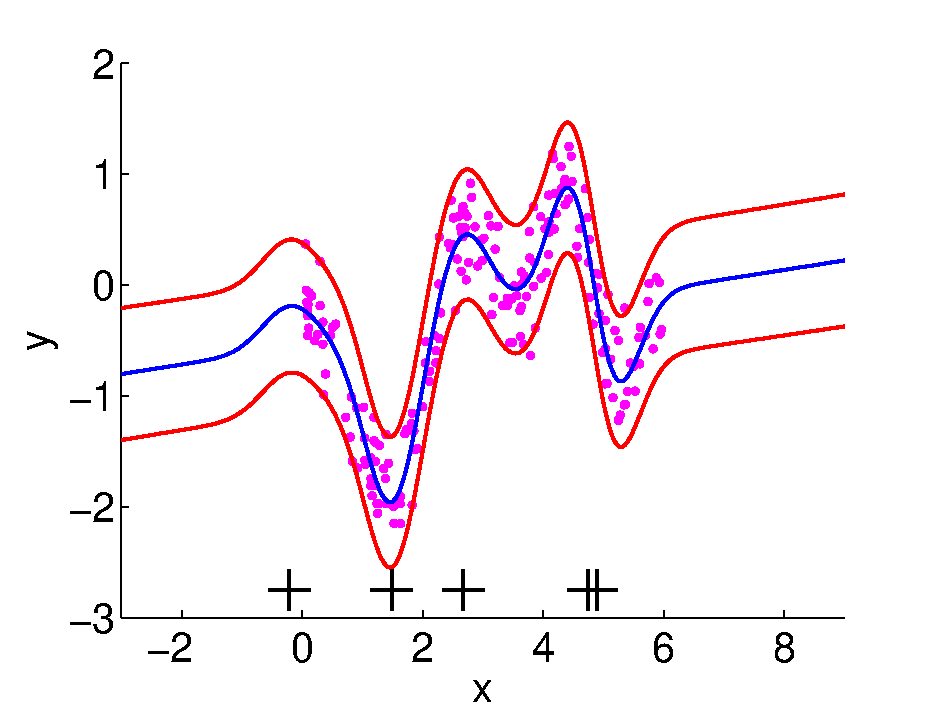
\includegraphics[scale=0.8]{../syn1/fig/syn_EigenGP_kerB_ns_M5_10.pdf}
\newpage
\section{Synthetic dataset 2}
\begin{table*}[h]
\caption{NMSE Results (M=15)} \label{table:basisfunction}
\vspace{-.0in}
\begin{center}
\begin{tabular}{|c|c|}
\hline
Methods & NMSE \\
\hline 
\hline
EigenGP (ARD) &  $ 0.051 \pm 0.0078$\\
\hline
EigenGP (ARD+linear)& $0.13\pm0.0027$ \\
\hline 
\end{tabular}
\end{center}
\vspace{-.0in}
\end{table*}

The composite model does not perform well on this dataset for (M=15). The following is the result of one run:

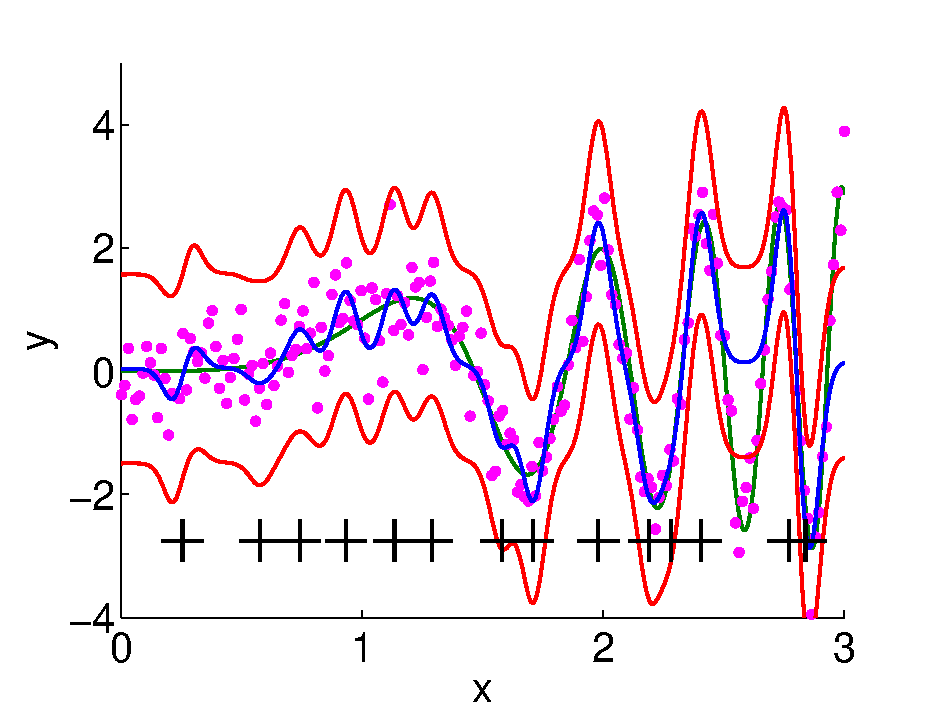
\includegraphics[scale=0.8]{../syn2/fig/syn_EigenGP_kerB_ns_8.pdf}


\end{document}
